\problemname{Skyltar}
\noindent
Efter att ha hört rykten om de otäcka muterade jätteråttorna i Göteborgs kloaker bestämde sig dina närmsta vänner att fly upp till det
underbara Stockholm. Under sin flykt märkte dina vänner att det märkligt nog fanns 
väldigt många vägskyltar längs vägen till Stockholm som pekade på olika små byar nere vid Lund. 
Dessutom verkade siffrorna på skyltarna vara lite suspiciösa, då vissa av skyltarna motsäger informationen som finns på andra skyltar.

På vardera av de $N$ vägskyltarna som dina vänner åkte förbi står det avstånden till alla $M$ byar i Lund. 
Avstånden är avrundade till närmaste heltal, då det faktiska avståndet inte nödvändigtvis är ett heltal. 
Eftersom dina goda vänner råkar ha perfekt fotografiskt minne, så kommer de ihåg exakt vilka avstånd som stod på skyltarna. 
Däremot minns dina vänner inte när eller i vilken ordning de såg dessa $N$ skyltar.

Du kan anta att Stockholm, Göteborg och de små byarna nere vid Lund alla ligger på en enda rak linje. 
Du kan dessutom anta att alla städer, byar och skyltar är så små att de kan representeras som punkter på denna linje.
Du kan även anta att ingen av Lunds byar ligger mellan två skyltar. Med andra ord ligger byarna i Lund och skyltarna på olika sidor av Göteborg.
Varken byarna eller skyltarna behöver vara placerade på heltalspositioner. 


\begin{centering}
  \begin{figure}[h]
      \centering
      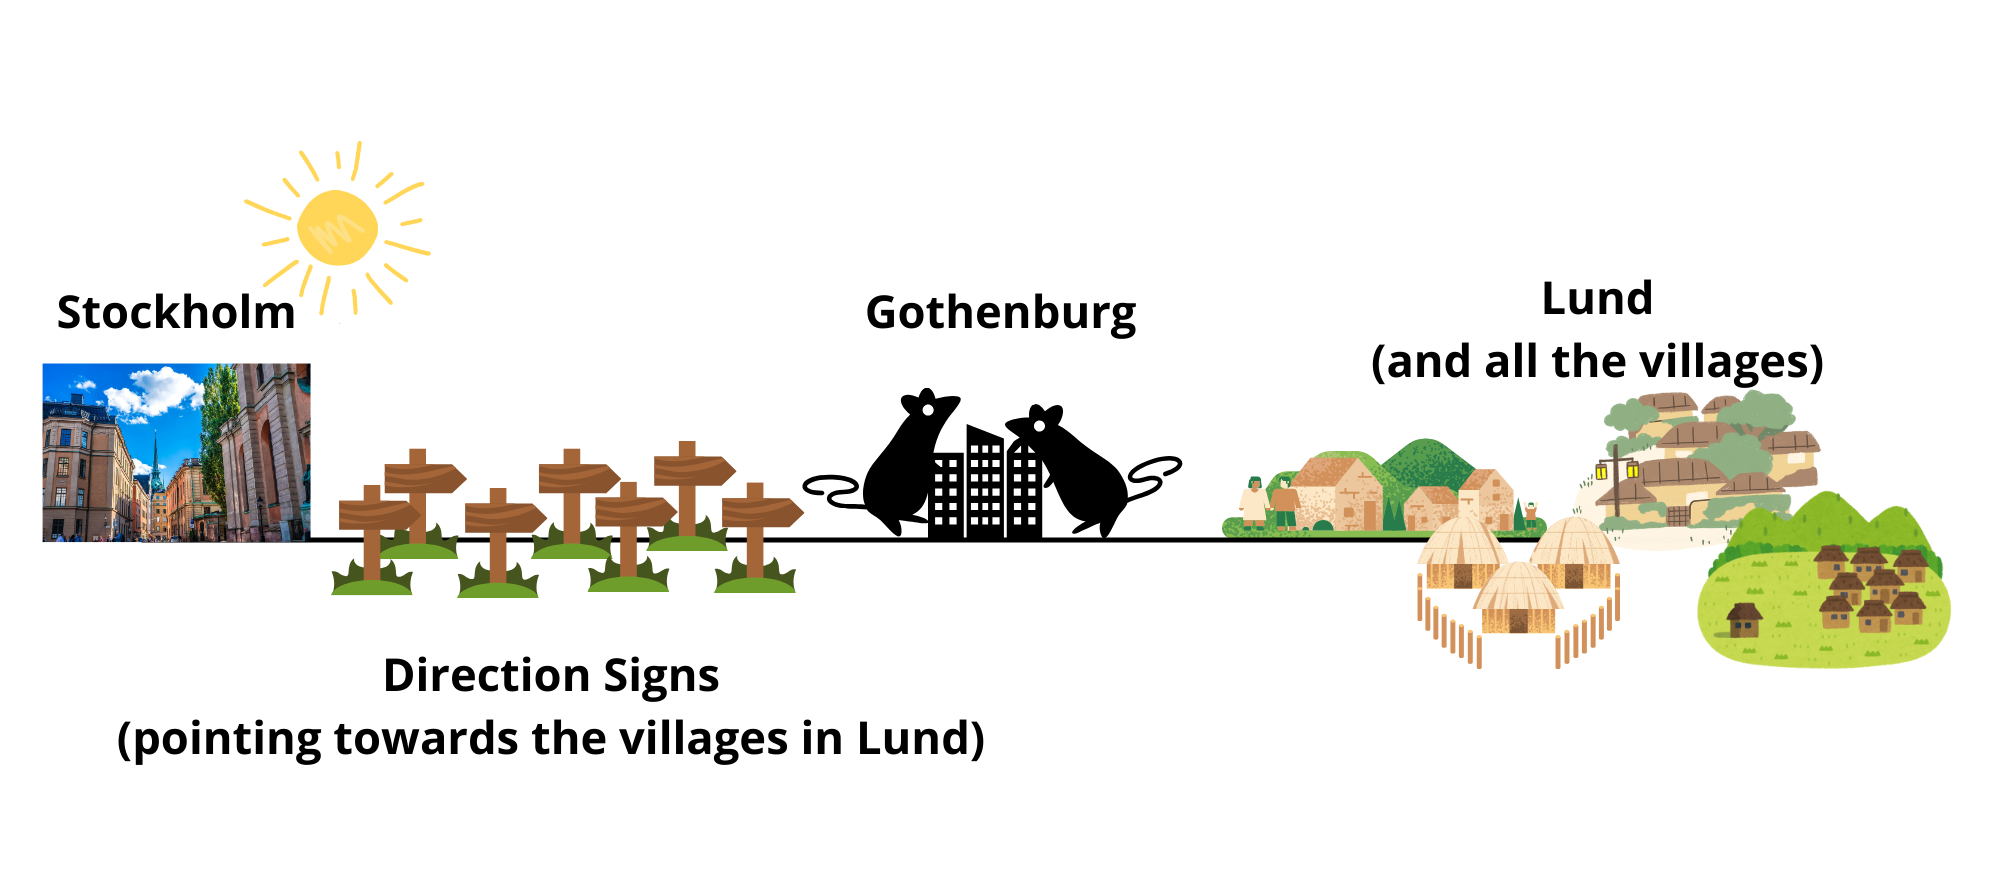
\includegraphics[width=0.8\textwidth]{skyltar.png}
      \caption{Bilden visar hur byarna i Lund och skyltarna befinner sig på olika sidor av Göteborg.}
  \end{figure}
\end{centering}

Givet dessa $N$ skyltar som dina vänner har sett, vad är det största mängden av dessa $N$ skyltar sådan att avståndet givna på skyltarna inte skapar några motsägelser? 
Slutligen kan du även anta att åtminstone $20\%$ av alla skyltar är helt korrekta, och inte orsakar några motsägelser.

\noindent
\section*{Indata}
Första raden innehåller två heltal $N$ och $M$ ($1 \leq N \leq 1000$, $1 \leq M \leq 200$),
som representerar antalet skyltar dina vänner har sett och antalet byar i Lund respektivt.

De följande $N$ raderna innehåller $M$ heltal vardera. Det $i$:te raden innehåller heltalen $d_{i,1}, d_{i,2}, \ldots, d_{i,M}$ ($1 \leq d_{i,j} \leq 10^6$) som beskriver de $M$ avstånden som står på den $i$:te skylten. 
På den $i$:te skylten står det alltså att avståndet från skylt $i$ till by $j$ avrundat nedåt blir $d_{i,j}$ för alla $1 \leq j \leq M$.


\section*{Utdata}
Skriv först ut ett heltal $t$, maximala antalet skyltar som är konsistenta. 
På nästa rad, skriv ut $t$ heltal som specifierar indexen i sorterad ordning sådan att den 
första skylten är den som är längst bort från Göteborg och alla byar i Lund, samt den sista skylten är närmast Göteborg och de mysiga byarna i Lund.
Eftersom folk i samhället blir förvirrade när saker är $0$-indexerade, vill vi att skyltarna är $1$-indexerade. Alltså är första skylten i input indexerad $1$, och sista skylten med index $N$.
Ifall det finns mer än ett svar kan ditt program skriva ut ett valfritt alternativ av dessa möjliga svar.

\section*{Poängsättning}
Din lösning kommer att testas på en mängd testfallsgrupper.
För att få poäng för en grupp så måste du klara alla testfall i gruppen.

\noindent
\begin{tabular}{| l | l | p{12cm} |}
  \hline
  \textbf{Grupp} & \textbf{Poäng} & \textbf{Gränser} \\ \hline
  $1$    & $21$         & $N \leq 15, M \leq 50$.  \\ \hline
  $2$    & $31$         & $N \leq 100, M \leq 50$ \\ \hline
  $3$    & $18$         & $N \leq 500, M \leq 50$ \\ \hline
  $4$    & $30$         & Inga ytterligare begränsningar. \\ \hline
\end{tabular}



\section*{Förklaring av första exempelfallet:}
Föreställ dig en tallinje på $x$-led.
Om vi tänker oss att den andra skylten är placerad på position $x = 1$, och den första sklylten på position $x = 1\frac{1}{2}$, 
den första byn på position $x = 3\frac{1}{2}$, och den andra byn $x = 4$. 

Det är även möjligt att hitta en konstruktion med skylt nr. 1 och 3.

Det är klart att sklyt nr. 1 och 2 motsäger varandra, vilket innebär att det inte finns en konstruktion där alla 3 skyltar används.

\section*{Kommentar till det andra exempelfallet:}
Notera att alla skyltar har avrundat ner avståndet till olika tal, trots att alla skyltar pekar på samma by.

\section*{Kommentar till det tredje exempelfallet:}
Notera att alla par av skyltar leder till en motsägelse; en godtycklig skylt skulle ge rätt svar på detta fall.
